\newpage
\section{Color image processing \buch{p.394}}
\subsection{Color fundamentals \buch{p.395}}
\begin{itemize}
	\item Humans can perceive thousands of colors but only about 20-30 shades of gray
	\item Color is often a great feature of object detection and extraction
	\item White light can be split into a spectrum of colors
	\item The human visual system (HVS) is quite complex, but basically, the cones are responsible for the color vision
	\begin{itemize}
		\item There are about 7 million cones which can be put into three categories
		\begin{itemize}
			\item $65\% $ are sensitive to red
			\item $33\% $ are sensitive to green
			\item $2\% $ are sensitive to blue
		\end{itemize}
		\item while their numbers vary widely, their sensitivity is quite similar
		\begin{itemize}
			\item Therefore, the blue cones are the most sensitive
			\item But the spatial resolution of red is much higher than that of blue
		\end{itemize}
	\end{itemize}
	\item Red, Green and Blue are called additive primary colors
	\item Magenta, Yellow and Cyan are called subtractive primary colors
	\item Humans often describe color using
	\begin{description}
		\item[Brightness:] Chromatic notation of intensity
		\item[Hue:] The dominant color
		\item[Saturation:] How much white light is mixed in with the pure color
	\end{description}
	\item The very useful HSI (Hue, Saturation, Intensity) color space is based on the color perception of humans	
\end{itemize}

The amount of red(X), green (Y) and blue (Z) needed to form a given color are called the tristimulus values.
A color can then be specified using its trichromatic coefficients x,y and z, which are normalized so that they sum to 1.
For any wavelength of light in the visible spectrum, these values can be read from tables that are the results from extensive experimentation.

\[
	x = \frac{X}{X+Y+Z} \qquad
	y = \frac{Y}{X+Y+Z} \qquad
	z = \frac{Z}{X+Y+Z}
\]



\subsection{Color models \buch{p.401}}
A color model is also called a color space or a color system. It allows colors to be represented in a well defined way, and depending on the task at hand, one model might be better suited than another.

\subsubsection{RGB model \buch{p.402}}
Based on the three primary colors of the HVS and the most used model as most color camera systems and monitors have these three channels.


\subsubsection{CMY and CMYK model \buch{p.406}}
These are models well suited for the primary colors of pigments, such as used in printing. The K stands for black, which, in theory can be mixed by summing up all subtractive primary colors, but for printing, the result tends to be a bit muddy, hence black is its own color. \\

If all color values have been normalized, the conversion from an RGB to a CMY image is achieved by
\begin{equation}
	\left[ \begin{array}{l} C \\ M \\ Y \end{array} \right] = \left[ \begin{array}{l} 1 \\ 1 \\ 1 \end{array} \right] - \left[ \begin{array}{l} R \\ G \\ B \end{array} \right]
\end{equation}

\subsubsection{The HSI Color Model \buch{p.407}}
The HSI Color Model is well suited for image processing algorithms.\\
\begin{minipage}{0.6\textwidth}
\begin{itemize}
	\item \textbf{H} - hue: information about color, determined by an angle from some reference point $\rightarrow$ usually an angle of $0^\circ$ at the red axis.
	\item \textbf{S} - saturation: length from the origin to the arbitrary color point
	\item \textbf{I} - intensity: given by the position of the plane on the vertical intensity axis.
\end{itemize}
\end{minipage}
\hspace{0.05\textwidth}
\begin{minipage}{0.35\textwidth}
	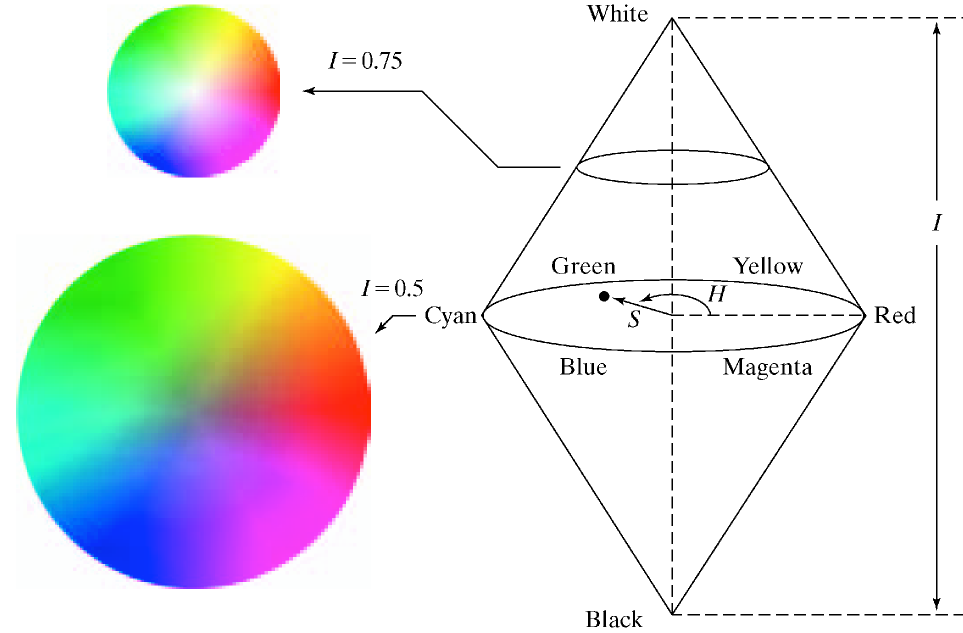
\includegraphics[width = \textwidth]{./images/HSI_ColorSpace}
\end{minipage}

\subsubsection{Converting RGB $\Rightarrow$ HSI \buch{p.410}}
The $H$ component of each RGB pixel is obtained by
\begin{equation}
	H = \begin{cases}
			\theta & \text{ if } B \leq G \\
			360 - \theta & \text{ if } B > G
		\end{cases}
\end{equation}
with
\begin{equation}
	\theta = \cos^{-1} \left[ \frac{\frac{1}{2} \left[ (R-G) + (R-B) \right]}{\left[(R-G)^2 + (R-B)(G-B)\right]^{1/2}} \right]
\end{equation}

The saturation component is given by
\begin{equation}
	S = 1 - \frac{3}{(R+G+B)} \left[ \min(R,G,B) \right]
\end{equation}

The intensity component is given by
\begin{equation}
	I = \frac{1}{3}(R+G+B)
\end{equation}

\subsubsection{Converting HSI $\Rightarrow$ RGB \buch{p.411}}
Given values of HSI in the interval $[0,1]$, the applicable equations depend on the values of $H$, according to the $120^{\circ}$ intervals separating the primaries.\\

First, $H$ is multiplied by $360^{\circ}$ so its range is $[0^{\circ},360^{\circ}]$. \\

\begin{tabularx}{\linewidth}{|l|X|X|X|}
	\hline 
	& \textbf{RG sector} ($0^{\circ} \leq H < 120^{\circ}$) & \textbf{GB sector} ($120^{\circ} \leq H < 240^{\circ}$) & \textbf{BR sector} ($240^{\circ} \leq H < 360^{\circ}$) \\ \hline
	$\mathbf{H}$ & $H = H$ & $H = H-120^{\circ}$ & $H = H-240^{\circ}$ \\ \hline
	$\mathbf{R}$ & $R = I \left[ 1 + \frac{S \cos(H)}{\cos(60^{\circ} - H)} \right]$ & $R = I(1-S)$ & $R = 3I - (R+B)$ \\
	$\mathbf{G}$ & $G = 3I - (R+B)$ & $G = I \left[ 1 + \frac{S \cos(H)}{\cos(60^{\circ} - H)} \right]$ & $G = I(1-S)$ \\
	$\mathbf{B}$ & $B = I(1-S)$ & $B = 3I - (R+B)$ & $B = I \left[ 1 + \frac{S \cos(H)}{\cos(60^{\circ} - H)} \right]$ \\
	\hline
\end{tabularx}


\subsection{Pseudo color image processing \buch{p.414}}
\begin{itemize}
	\item Assigning colors to gray values, based on a specified criterion.
	\item Goal: better human visualization and interpretation. \\
			Reason: humans can perceive thousands of color shades, but only 20-30 shades of gray.
\end{itemize}

\subsubsection{Intensity Slicing \buch{p.415}}
A gray-scale image with $[0,L-1]$ values is sliced into $P$ planes at the intensity levels $l_1,l_2,\dots,l_P$, creating the $P+1$ intervals $V_1,V_2,\dots,V_{P+1}$. Intensity to color assignments are made according to
\begin{equation}
	f(x,y) = c_k \qquad \qquad \text{if } f(x,y) \in V_k
\end{equation}
where $c_k$ is the color associated with the $k$th intensity interval $V_k$.

\subsubsection{Intensity to color transformation \buch{p.418}}
\begin{minipage}{12cm}
	A more general way than image slicing is to perform three independent transformations on the intensity. This method produces an image, whose color content is modulated by the transformation functions, which are only dependent on the intensity values.
\end{minipage}
\begin{minipage}{6cm}
	\adjustbox{width=6cm}{\begin{tikzpicture}
\tikzstyle{gray_block} = [draw,outer sep=0,inner sep=5,minimum width=110,minimum height=40,line width=1, very thick, draw=black!55, top color=white,bottom color=black!20]
\tikzstyle{vecArrow} = [thick, decoration={markings,mark=at position
   1 with {\arrow[semithick]{open triangle 60}}},
   double distance=1.4pt, shorten >= 5.5pt,
   preaction = {decorate},
   postaction = {draw,line width=1.4pt, white,shorten >= 4.5pt}]
\tikzstyle{innerWhite} = [semithick, white,line width=1.4pt, shorten >= 4.5pt]   
   
	\node (a) at (0,0) {$f(x,y)$};
	\node[inner sep=0,minimum size=0] (a1) at (1,0) {};
	\node (b) [gray_block] at (4,2) {Red transformation};
	\node (c) [gray_block] at (4,0) {Green transformation};
	\node (d) [gray_block] at (4,-2) {Blue transformation};
	\node (e) at (7.5,2) {$f_R(x,y)$};
	\node (f) at (7.5,0) {$f_G(x,y)$};
	\node (g) at (7.5,-2) {$f_B(x,y)$};

	\draw[vecArrow] (a)  -- (c);
	\draw[vecArrow] (a1) |- (b) ;
	\draw[vecArrow] (a1) |- (d) ;
	
	\draw[innerWhite] (a) |- (c);
	\draw[innerWhite] (a1) |- (b);
	\draw[innerWhite] (a1) |- (d);
	
	\draw[vecArrow] (b)  -- (e);
	\draw[vecArrow] (c)  -- (f);
	\draw[vecArrow] (d)  -- (g);
	
\end{tikzpicture}}
\end{minipage}

\subsection{Full-Color Image Processing \buch{p.424}}
In the RGB system, each point is represented by a vector
\begin{equation}
	c = \left[\begin{array}{l}
		c_R \\ c_G \\ c_B
	\end{array} \right]
	= \left[\begin{array}{l}
		R \\ G \\ B
	\end{array} \right]
	\qquad \text{thus an image is represented by} \qquad
	c(x,y) = \left[\begin{array}{l}
		c_R(x,y) \\ c_G(x,y) \\ c_B(x,y)
	\end{array} \right]
	= \left[\begin{array}{l}
		R(x,y) \\ G(x,y) \\ B(x,y)
	\end{array} \right]	
\end{equation}

\subsection{Color Transformations \buch{p.426}}
Color transformations describe processing of a color image within a \textit{single} color model. Any transformation can be performed in any color model, howere some operations are better suited to specific models. \\

Generally a transformation is described by 
\begin{equation}
	g(x,y) = T\left[f(x,y)\right]
\end{equation}
where $T$ is an operator on $f$ over a spatial neighborhood. Each pixel value is a triplet or quartet. \\

\subsubsection{Color complements \buch{p.430}}
\begin{minipage}{12cm}
	The hues directly opposite one another are called \textit{complements}. They are analogous to the gray-scale negatives and are useful for enhancing details. The transformations can be achieved in the RGB or the HSI color spaces using the transfer functions shown on the right.
\end{minipage}
\begin{minipage}{6cm}
	\centering
	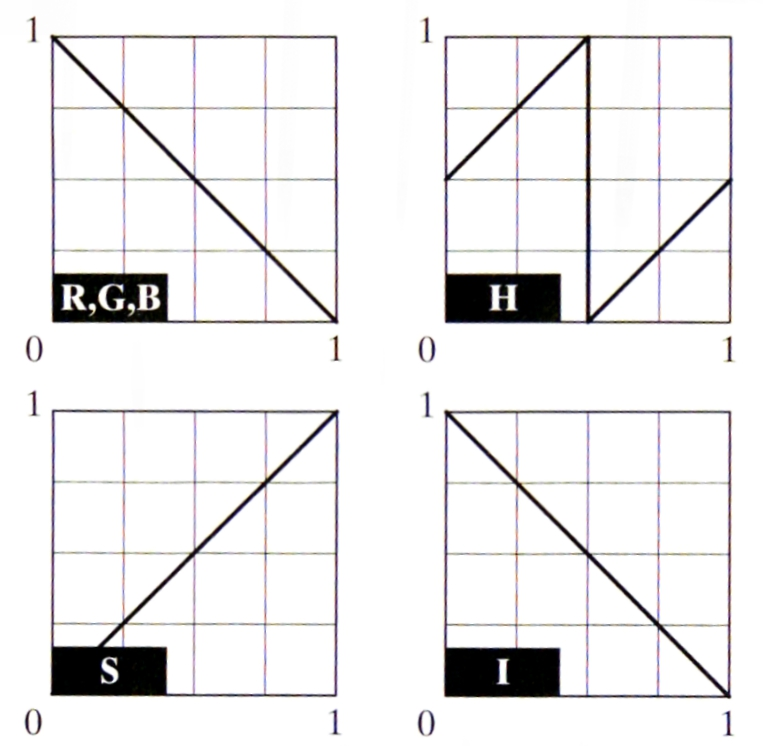
\includegraphics[width=4cm]{images/ColorComplements.jpeg}
	%TODO: vertikzisieren und evtl. anders anordnen
\end{minipage}

\subsubsection{Color slicing \buch{p.431}}
Color slicing is used to highlight a specific range of colors, to separate objects from their surroundings. A simple way to achieve this is to map the $n$ color-components (usually 3 or 4) outside a cube of width $W$, centered at $(a_1,a_2,\dots,a_n)$, to a neutral color (e.g. gray = $(0.5,0.5,0.5)$ in RGB), by
\begin{equation}
	s_i = \begin{cases}
		0.5 & \text{  if } \left[ \left| r_j - a_j \right| > \frac{W}{2} \right]_{\text{any } 1 \leq j \leq n} \\
		r_i & \text{  otherwise}
	\end{cases} \qquad \qquad i = 1,2,\dots,n
\end{equation}

Similarly, any region can be used. A sphere with radius $R_0$ and center $(a_0,a_1,\dots,a_n)$ is given by
\begin{equation}
	s_i = \begin{cases}
		0.5 & \text{  if } \sum_{j=1}^{n} (r_j - a_j)^2 > R_0^2 \\
		r_i & \text{  otherwise}
	\end{cases} \qquad \qquad i = 1,2,\dots,n
\end{equation}

\subsection{Tone and Color Corrections \buch{p.433}} 
%TODO: How relevant is this anyway?
Used for photo enhancement and color reproduction. Most tone and color corrections are performed using a \textit{device-independent color model}, such as the CIE $L^* a^* b^*$ model given by
\begin{align}
	L^* &= 116 \cdot h(\frac{Y}{Y_W}) - 16 \\
	a^* &= 500 \left[ h(\frac{X}{X_W}) - h(\frac{Y}{Y_W}) \right] \\
	b^* &= 200 \left[ h(\frac{Y}{Y_W}) - h(\frac{Z}{Z_W}) \right]
\end{align}

where
\begin{equation}
	h(q) = \begin{cases}
		\sqrt[3]{q} & q > 0.008856 \\
		7.787q + 16/116 & q \leq 0.008856
	\end{cases}
\end{equation}
and $X$ represents red, $Y$ represents green and $Z$ represents blue in the XYZ color space. $X_W$,$Y_W$,$Z_W$ are reference white values, typically the white of a perfectly reflecting diffuser under CIE standard D65 illumination. \\

$L^*$ represents lightness, $a^*$ red minus green and $b^*$ green minus blue, making it useful in image manipulation and image compression.

\subsubsection{Histogram Processing \buch{p.438}}
It is generally unwise to apply histogram equalization to the components of a color image independently. Usually, the color intensities are spread uniformly, leaving the colors unchanged. The HSI color spaced is ideally suited to this type of approach.

\subsection{Smoothing and sharpening \buch{p.439}}
\subsubsection{RGB Color Space}
In the RGB color space, image smoothing can be carried out per-color-plane by
\begin{equation}
	\overline{c}(x,y) = \left[ \begin{array}{l}
		\frac{1}{K} \displaystyle\sum_{(s,t) \in S_{xy}} R(s,t) \\
		\frac{1}{K} \displaystyle\sum_{(s,t) \in S_{xy}} G(s,t) \\
		\frac{1}{K} \displaystyle\sum_{(s,t) \in S_{xy}} B(s,t) \\
	\end{array} \right]
\end{equation}

Similarly, image sharpening can be achieved using the Laplacian on each component of the color vector
\begin{equation}
	\nabla^2 \left[ c(x,y) \right] = \left[ \begin{array}{l}
		\nabla^2 R(x,y) \\
		\nabla^2 G(x,y) \\
		\nabla^2 B(x,y) \\		
	\end{array} \right]
\end{equation}

\subsection{HSI Color Space}
The HSI color space decouples intensity and color information, so image smoothing can be achieved by simply smoothing the intensity component. The result will not be exactly the same as in the RGB color space, as only the intensity is changed but not hue and saturation. \\

Similarly, image sharpening can be achieved by applying the Laplacian operator on the intensity component and leaving hue and saturation unchanged.

\subsection{Image segmentation based on color \buch{p.443}}
In the HSI space, image segmentation can be achieved by multiplying the hue with a binary mask, generated by thresholding the saturation image, resulting in a hue image. By selecting only the desired hues with a threshold, the image can be segmented. \\

Segmentation in the RGB space normally yields better results:

Let $\mathbf{a}$ be the average color, one tries to segment. $\mathbf{z}$ denotes an arbitrary point. If the distance between $\mathbf{a}$ and $\mathbf{z}$ is below a specific threshold $D_0$, the colors are \textit{similar}. 

\begin{equation}
	D(\mathbf{z},\mathbf{a}) = \left|\left| \mathbf{z}-\mathbf{a} \right|\right| = \left[(\mathbf{z}-\mathbf{a})^T(\mathbf{z}-\mathbf{a})\right]^{1/2} = \left[ (z_R-a_R)^2 + (z_G-a_G)^2 + (z_B-a_B)^2 \right]^{1/2}
\end{equation}

If $D(\mathbf{z},\mathbf{a}) \leq D_0$, the color is inside a sphere of radius $D_0$ around $\mathbf{a}$. 

\subsubsection{Bounding boxes \buch{p.446}}
As the computation of the above is rather expensive, even if the square roots aren't computed, a compromise is to use a bounding box centered on $\mathbf{a}$, with dimensions along each of the color axes chosen proportional to the standard deviation of the samples along each of the axis.

\subsection{Color edge detection \buch{p.447}}
Two possibilities to detect edges in RGB-color space:
\begin{enumerate}
	\item Use Sobel operators on each color to form the gradient of each RGB component and add them together at each coordinate (x,y)
	\item Vector method described on p.449
\end{enumerate}

\subsection{Noise in color images \buch{p.451}}
Some of the gray scale methods are allowed for full color images.

Other schemes cannot be that easily extended to color images, such as the order statistic filters.